\chapter{User evaluation}
\label{chap:user-evaluation}

\note{NOT READY YET!!}

This chapter presents the last (and most extensive) experiment carried out in the course of this thesis. The empirical studies exposed so far in Chapters \ref{chap:wozlearning} and \ref{chap:rllearning} essentially focused on the learning performance of rule-structured models compared to more classical representations. But albeit such empirical measures can provide useful insights about the model adequacy for various dialogue domains, they are not by themselves sufficient to assess the suitability of a particular modelling approach and its practical effects on the quality of the produced interactions. 

In order to corroborate our claims regarding the benefits of structured probabilistic modelling for dialogue management and contrast it to traditional approaches, we conducted an user evaluation experiment with a total of \note{xxx} users. The aim of the experiment was to compare three alternative approaches to dialogue management (two baselines and our own approach) in an human--robot interaction domain.  The three approaches respectively correspond to a purely handcrafted approach, a purely statistical approach, and a hybrid approach based on probabilistic rules. 

The collected interactions were subsequently analysed to extract various metrics of interaction quality and efficiency.  The metrics included both objective measures such as the number of errors, clarification requests, and task outcome, but also subjective measures of user satisfaction, based on a survey completed by the participants after each interaction. \note{give here a teaser about the results}

\note{The chapter is structured in four sections: ...}

\section{Interaction scenario}

The interaction scenario employed for the user evaluation is similar in most respects to the one presented in Section \ref{sec:rllearning-experiments}, but has been adapted (as a follow-up to the feedback provided by some participants) to circumscribe more precisely the task that is to be performed. 

A Nao robot stands on a large table and can move around across the table, as illustrated in Figure \ref{fig:scenario}.  The purpose of the interaction is to instruct the robot to (1) move to the other side of the table without bumping into the (imaginary) walls, (2) pick up one of the object, (3) bring it back to the left side of the table, and (4) release it at a specific landmark. 

The robot can perceive the presence, colour and location of each physical object thanks to visual markings placed at their top.  It can also grasp each object with the help of permanent magnets fixed on the hands of the robot. 

\begin{figure}[h]
\vspace{3mm}
\centering
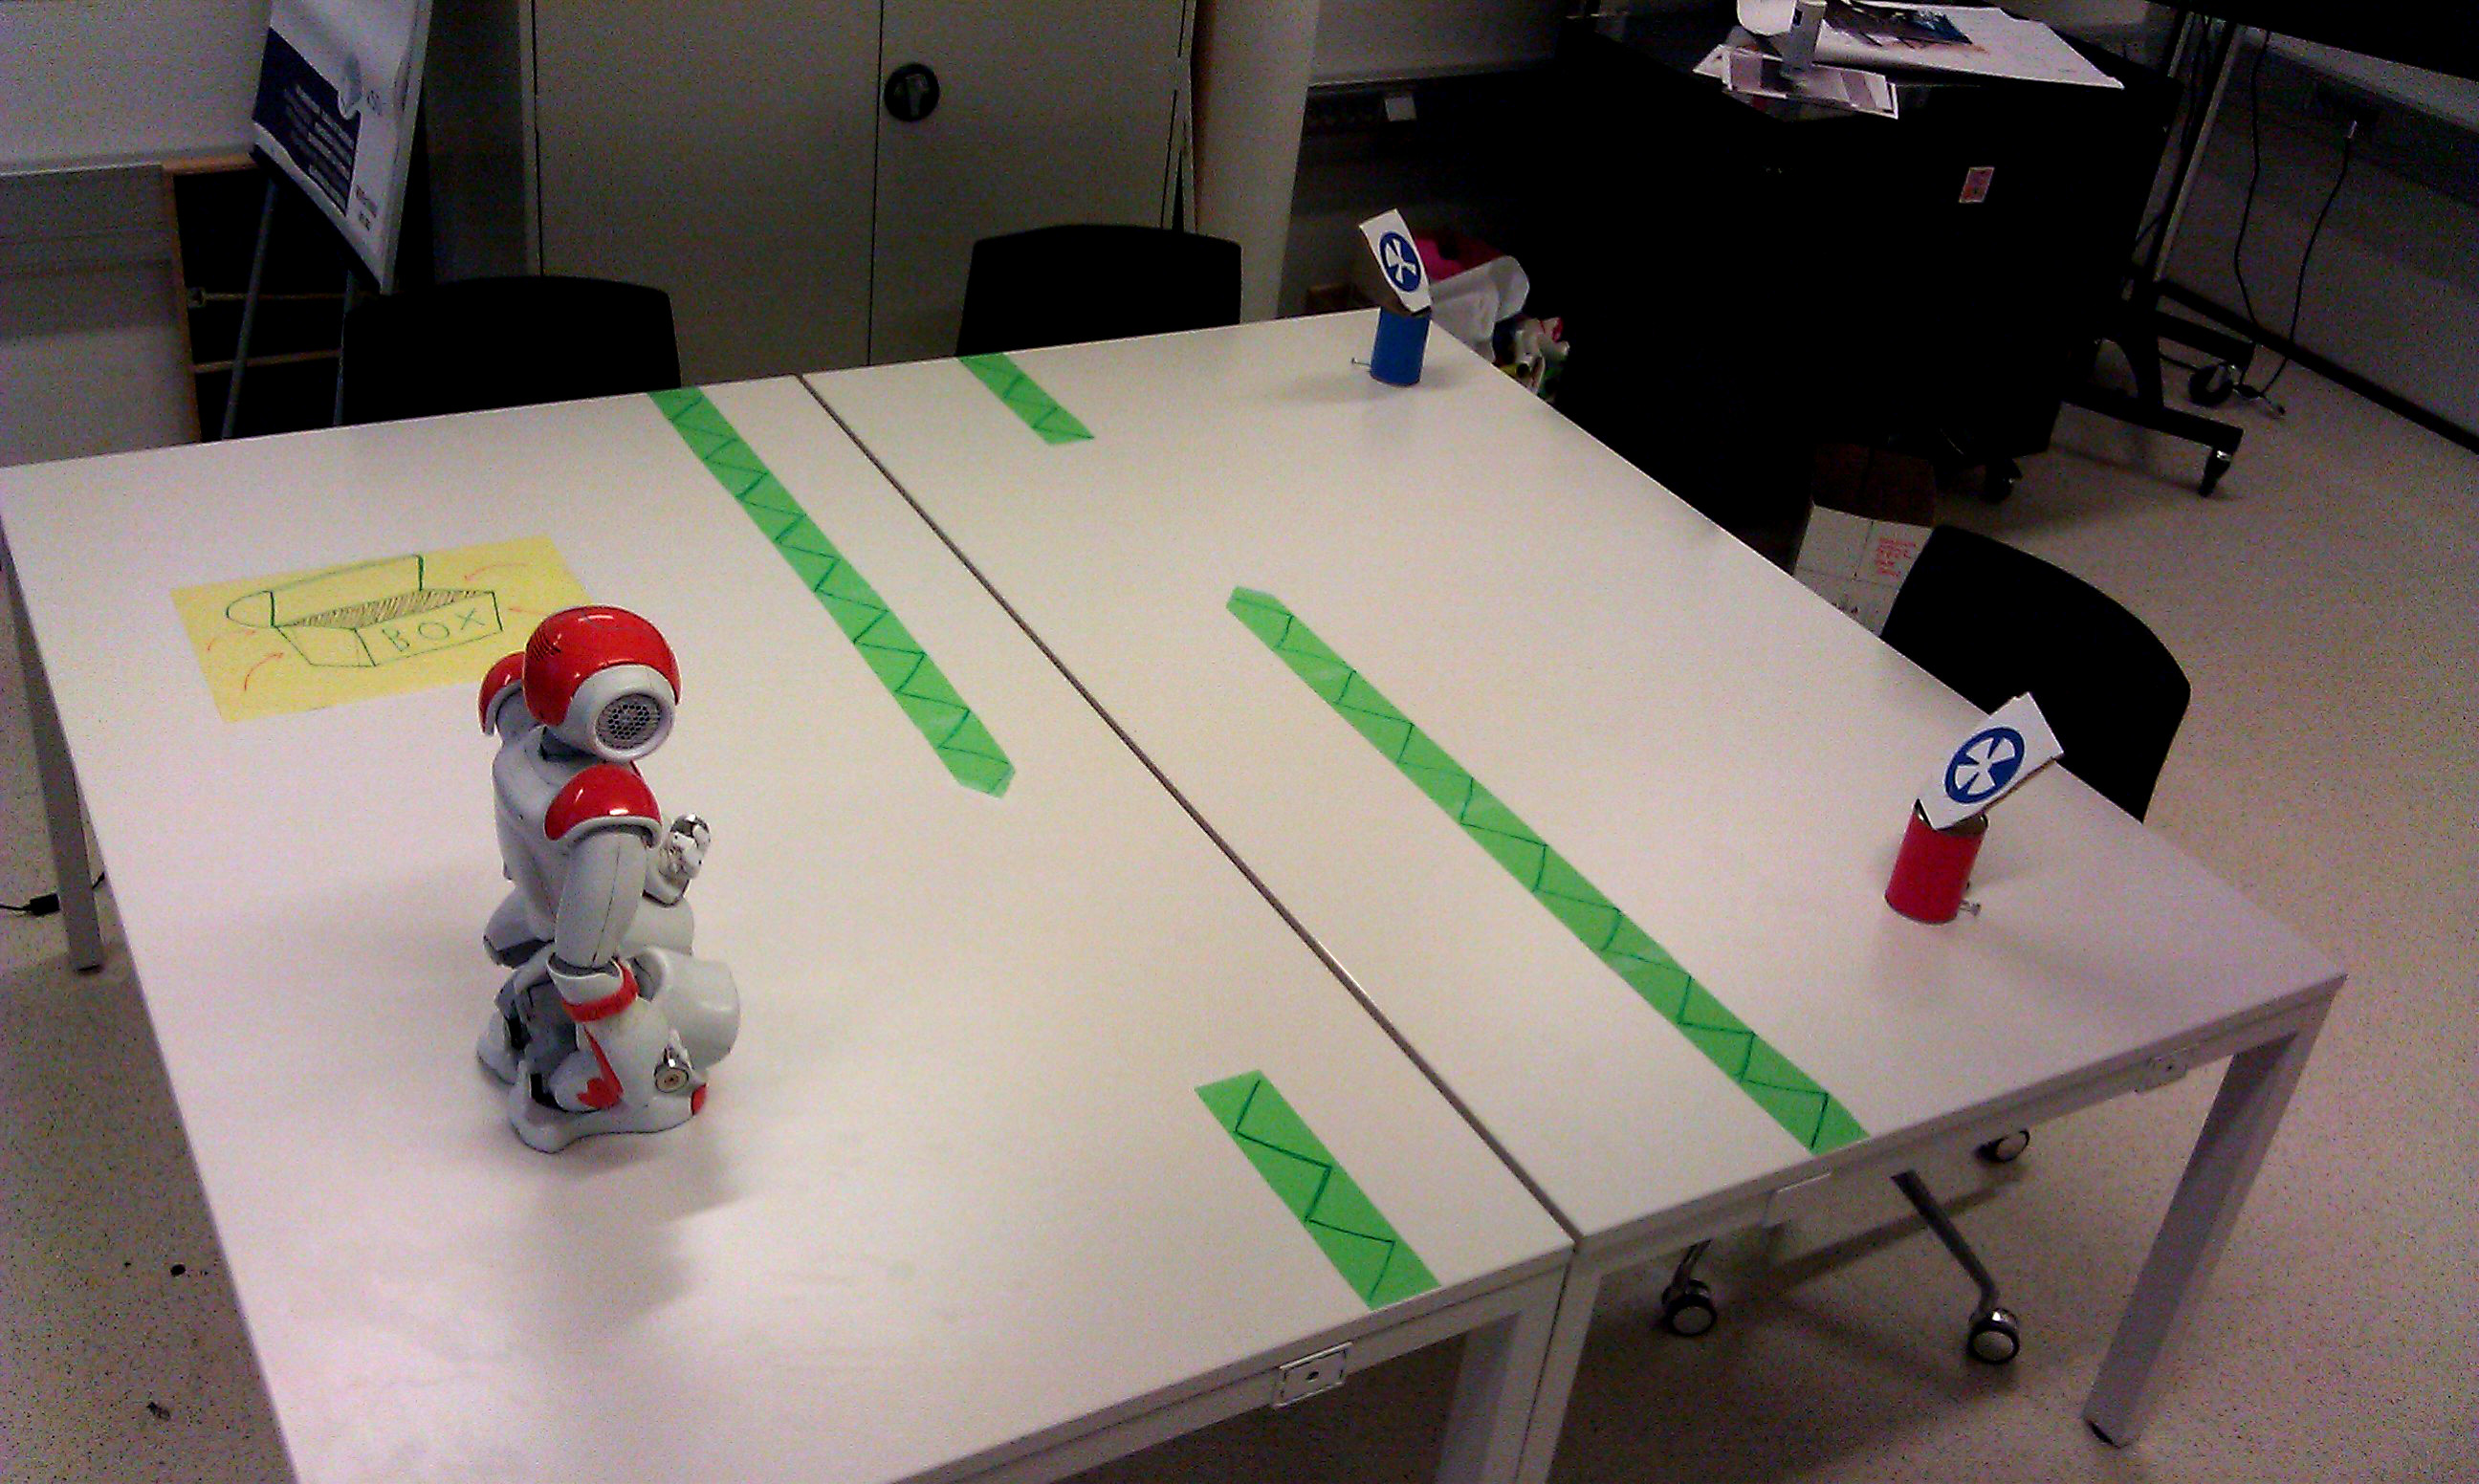
\includegraphics[scale=0.13]{imgs/scenario.jpg} \vspace{3mm}
\caption{Interaction scenario for the experiment.  On the right side of the table stand two objects (one red and one blue).  Imaginary walls (in green) are also placed on the table, as well as a yellow landmark depicting the final destination of the robot. }
\label{fig:scenario}
\end{figure}


\subsection{Dialogue domain}

\subsubsection*{User intentions and actions}

As for the previous experiment, we represent each basic instruction (such as moving forward, turning left, picking up an object, etc.) as a distinct user intention $i_u$. After the fulfilment of each instruction, the user intention is reinitialised to represent the next instruction to perform.  The possible user intentions for the domain are shown in Table \ref{table:userintents_exp3}.  

A few changes can be noted compared to the Wizard-of-Oz study presented in Section \ref{sec:rllearning-experiments}.  First, the basic movements are now completed with a second argument specifying the duration of the movement, e.g. short or long. The human user can therefore explicitly request the robot to perform a short or long movement. A new type of movement has also been added, $\mathrm{Move(Turn)}$ to make the robot turn around by 180 degrees.  Finally, specific intentions are used to capture the opening (engagement) and closing (disengagement) phases of the dialogue. 

The possible user actions $a_u$, listed in Table \ref{table:userdas_exp3} are a reflection of these user intentions. The user can directly utter an instruction, ask the robot to repeat its last movement, or respond to a clarification or confirmation request. Two new additions are the user action $\mathrm{Ask(Stop)}$ to tell the robot to stop its current movement, and the grounding action $\mathrm{Grounding}$ to represent explicit positive feedback provided by the user on the robot behaviour.

\subsubsection*{System actions}
As shown in Table \ref{table:systemdas_exp3}, the system actions $a_m$ include: \begin{itemize}
\item Physical movements to move around in various directions and lengths, pick up or put down physical objects on the table, or stop the current move.
\item Verbal responses to the user's requests, in order to confirm or deny the detection of a particular object, describe the robot's current perception, or tell the user that it cannot perform a requested movement due to some impeding factor (e.g. not being able to pick up an object whose location is currently not known). 
\item Clarification and confirmation requests, such as asking the user to repeat her/his last utterance, or confirming a particular intention.
\end{itemize}

Instead of representing grounding actions in a separate category of actions (as in Table \ref{table:systemdas_exp2}), the grounding acts are now directly coupled to the system actions. The selection of the system action $\mathrm{Do}(x)$ therefore triggers both a grounding action (\utt{Ok, now doing $x$}) and the simultaneous execution of the corresponding physical movement. 

\renewcommand{\arraystretch}{1.3}

\begin{table}[p!]
\begin{footnotesize}
\begin{tabular}{p{60mm}} 
$\cdot$ $\mathrm{Move}(x,y) $ \\ $ \ \ \ \ \ \text{ where } x=\{\mathrm{Left,Right,Forward,}$ \\ $\ \ \ \ \ \ \ \ \ \ \ \ \ \ \ \ \ \ \ \ \ \ \ \ \ \mathrm{Backward}\} $ \\ $ \ \ \ \ \ \ \text{ and } y = \{\mathrm{Short, Long}\}$ \\
$\cdot$ $\mathrm{Move(Turn)} $ \\
$\cdot$ $\mathrm{PickUp}(x) $ \\ $\ \ \ \ \  \text{ where } x \text{ is an object identifier}$ 
\end{tabular}
\hspace{2cm}
\begin{tabular}{p{60mm}} 
$\cdot$ $\mathrm{ReleaseObject} $ \\
$\cdot$ $\mathrm{WhatDoYouSee}$ \\
$\cdot$ $\mathrm{DoYouSee}(x) $ \\ $\ \ \ \ \  \text{ where } x \text{ is an object identifier}$ \\
$\cdot$ $\mathrm{Greeting}$ \\
$\cdot$ $\mathrm{Closing}$ 
\end{tabular}
\end{footnotesize}
 \caption{List of user intentions $i_u$} 
\label{table:userintents_exp3}
\end{table}


\begin{table}[p!]
\begin{footnotesize}
\begin{tabular}{p{60mm}} 
$\cdot$ $\mathrm{Ask(Move(x,y))} $ \\ $ \ \ \ \ \ \text{ where } x=\{\mathrm{Left,Right,Forward,}$ \\ $\ \ \ \ \ \ \ \ \ \ \ \ \ \ \ \ \ \ \ \ \ \ \ \ \ \mathrm{Backward}\} $ \\ $ \ \ \ \ \ \ \text{ and } y = \{\mathrm{Short,Long}\}$ \\
$\cdot$ $\mathrm{Ask(Move(Turn))} $ \\
$\cdot$ $\mathrm{Ask(PickUp(x))} $ \\ $\ \ \ \ \  \text{ where } x \text{ is an object identifier}$ \\ $\ \ \ \ \  \text{ or }  \mathrm{Other} \text{ if the reference is not resolved}$ \\
$\cdot$ $\mathrm{Ask(ReleaseObject)} $ \\
$\cdot$ $\mathrm{RepeatLast}$ \\
$\cdot$ $\mathrm{Ask(Stop)}$ 
\end{tabular}
\hspace{2cm}
\begin{tabular}{p{60mm}} 
$\cdot$ $\mathrm{Ask(WhatDoYouSee)}$ \\
$\cdot$ $\mathrm{Ask(DoYouSee(x))} $ \\ $\ \ \ \ \  \text{ where } x \text{ is an object identifier }$ \\ $\ \ \ \ \  \text{ or }  \mathrm{Other} \text{ if the reference is not resolved}$ \\
$\cdot$ $\mathrm{Confirm}$ \\
$\cdot$ $\mathrm{Disconfirm}$ \\
$\cdot$ $\mathrm{Grounding}$ \\
$\cdot$ $\mathrm{Greet}$ \\
$\cdot$ $\mathrm{Close}$ \\
$\cdot$ $\mathrm{Other}$ 
\end{tabular}
\end{footnotesize}
 \caption{List of user actions $a_u$} 
\label{table:userdas_exp3}
\end{table}

\begin{table}[p!]
\begin{footnotesize}
\begin{tabular}{p{60mm}} 
$\cdot$ $\mathrm{Do}(x) $ \\ $ \ \ \ \text{ where } x=\{\mathrm{Move}(y,z), \mathrm{Move(Turn)},$ \\ $\ \ \ \ \ \ \ \ \ \ \ \ \ \ \ \ \ \ \ \ \ \ \ \mathrm{PickUp}(a),  \mathrm{ReleaseObject},$ \\ $\ \ \ \ \ \ \ \ \ \ \ \ \ \ \ \ \ \ \ \ \ \ \ \mathrm{Stop}\} $ \\ $ \ \ \ \ \ \ \text{ and } y = \{\mathrm{Left,Right,Forward,}$ \\ $ \ \ \ \ \ \ \ \ \ \ \ \ \ \ \ \ \ \ \ \ \ \ \ \mathrm{Backward}\} $ \\ $ \ \ \ \ \ \ \text{ and } z = \{\mathrm{Short,Long}\}$ \\ $ \ \ \ \ \ \  \text{ and } a = \ \text{an object identifier}$ \\
$\cdot$ $\mathrm{Excuse}(x) $ \\ $ \ \ \  \text{ where } x = \{\mathrm{UnseenObject}$ \\ $\ \ \ \ \ \ \ \ \ \ \ \ \ \ \ \ \ \ \ \ \ \ \ \mathrm{UnresolvedReference},$  \\ $\ \ \ \ \ \ \ \ \ \ \ \ \ \ \ \ \ \ \ \ \ \ \ \mathrm{NoCarriedObject,}$ \\ $\ \ \ \ \ \ \ \ \ \ \ \ \ \ \ \ \ \ \ \ \ \ \ \mathrm{AlreadyCarryObject}\}$ \\
$\cdot$ $\mathrm{Greet}$ \\
$\cdot$ $\mathrm{Goodbye}$ 
\end{tabular}
\hspace{2cm}
\begin{tabular}{p{60mm}} 
$\cdot$ $\mathrm{Describe}(x) $ \\ $ \ \ \  \text{ where } x = \ \text{a (possibly empty) list}$ \\ $ \ \ \ \ \ \ \ \ \ \ \ \ \ \ \ \ \ \ \ \ \ \ \  \text{of object identifiers}$ \\
$\cdot$ $\mathrm{ConfirmDetection}$ \\
$\cdot$ $\mathrm{DisconfirmDetection}$  \\
$\cdot$ $\mathrm{AskClarify}$ \\
$\cdot$ $\mathrm{AskConfirm}(x) $\\ $ \ \ \ \text{ where } x=\{\mathrm{Move}(y,z), \mathrm{Move(Turn)},$ \\ $\ \ \ \ \ \ \ \ \ \ \ \ \ \ \ \ \ \ \ \ \ \ \ \mathrm{PickUp}(a),  \mathrm{ReleaseObject},$ \\ $\ \ \ \ \ \ \ \ \ \ \ \ \ \ \ \ \ \ \ \ \ \ \ \mathrm{Stop}\} $ \\ $ \ \ \ \ \ \ \text{ and } y = \{\mathrm{Left,Right,Forward,}$ \\ $ \ \ \ \ \ \ \ \ \ \ \ \ \ \ \ \ \ \ \ \ \ \ \ \mathrm{Backward}\} $ \\ $ \ \ \ \ \ \ \text{ and } z = \{\mathrm{Short,Long}\}$ \\ $ \ \ \ \ \ \  \text{ and } a = \ \text{an object identifier}$ \end{tabular}
\end{footnotesize}
 \caption{List of system actions $a_m$} 
\label{table:systemdas_exp3}
\end{table}

\subsubsection*{Dialogue state}

The dialogue state $\mathcal{B}$ chosen for the dialogue domain is factored in eleven distinct state variables, encoding both the user intentions and actions, the external context, the recent interaction history, and the physical status of the robot. Table \ref{table:statevariables} details the name, purpose, range of possible values, observability and dependencies of each state variable. 

One can distinguish in this table three distinct types of state variables:
\begin{enumerate}
\item State variables such as $u_u$, $\mathit{perceived}$, $\mathit{carried}$ and $\mathit{motion}$ represent \textit{observations} arising from the robot sensors and speech recognition engine. Observations such as $\mathit{carried}$ and $\mathit{motion}$ are (near-)certain, while the last user utterance and the set of perceived objects are uncertain observations expressed through categorical distributions over alternative values. 
\item State variables such as $i_u$, $a_u$, $a_{u\mbox{-}prev}$ and $\mathit{completed\mbox{-}task}$ are essentially \textit{hidden variables}. Hidden variables are always expressed as categorical distributions and are indirectly inferred from the accumulated observations and actions.
\item Finally, variables such as $a_m$, $u_m$ and $\mathit{lastMove}$ represent (present or past) \textit{decisions} made by the system. These decisions are naturally known to the system and are thus fully observed. 
\end{enumerate}

Even when abstracting from the two variables $u_u$ and $u_m$ (which have a virtually infinite set of possible values, as they can accept any string) and assuming the presence of only two objects, the total size of the joint state space is a non-trivial one to tackle: 
\begin{align}
|\mathcal{S}| & = & 4 &&& [\text{size of } Val(\mathit{perceived})] \nonumber \\
 && \times 3 &&&  [\text{size of } Val(carried)] \nonumber \\
 && \times 18 &&&  [\text{size of } Val(i_u)] \nonumber \\
&&  \times 25 &&&  [\text{size of } Val(a_u)] \nonumber \\
&&  \times 25 &&&  [\text{size of } Val(a_{u\mbox{-}prev})] \nonumber \\
&&  \times 41 &&&  [\text{size of } Val(a_m)] \nonumber \\
&&  \times 2 &&&  [\text{size of } Val(\mathit{motion})] \nonumber \\
&&  \times 14 &&&  [\text{size of } Val(\mathit{lastMove})] \nonumber \\
&&  \times 2 &&&  [\text{size of } Val(\mathit{completed\mbox{-}task})] \nonumber \\
 & =  & 30 \ 9960 \ 000 &&& \nonumber 
  \end{align}
 
\renewcommand{\arraystretch}{1.9}
\setlength{\tabcolsep}{8pt}
\begin{sidewaystable}
\begin{center}
\begin{tabular}{|p{35mm}||p{7cm}p{5mm}|p{34mm}p{5mm}|p{27mm}|p{4cm}|} \hline
\textbf{Variable label:} & \textbf{Description:}  && \textbf{Range of values:} && \textbf{Observability: } & \textbf{Dependencies: }\\ \hline\hline
$\mathit{perceived}$ & Objects perceived in the visual field && (possibly empty) set of object identifiers && Partial& $\emptyset$ \\\hline
$\mathit{carried}$ & Object carried by the robot && (possibly empty) set of object identifiers && Full  & $\emptyset$ \\\hline
$i_u$ & Current user intention && cf. Table \ref{table:userintents_exp3} && Partial  & $\mathit{completed\mbox{-}task}$, $\mathit{perceived}$, $\mathit{carried}$ \\\hline
$u_u$ & Last user utterance && ASR hypotheses && Partial & $\emptyset$ \\ \hline
$a_u$ & Last dialogue act from the user && cf. Table \ref{table:userdas_exp3} && Partial & $u_u$, $i_u$, $a_m$, $\mathit{lastMove}$ \\\hline
$a_{u\mbox{-}prev}$ & Next-to-last dialogue act from the user && cf. Table \ref{table:userdas_exp3} && Partial & $\emptyset$ \\\hline
$a_m$ & Last system action && cf. Table \ref{table:systemdas_exp3} && Full & $i_u$, $a_u$, $\mathit{motion}$, \ \ \ \ \  $\phantom{a}$ $\mathit{perceived}$, $\mathit{carried}$ \\ \hline
$\mathit{motion}$ & Activity status of the robot (denoting whether the robot is currently moving) && $\mathit{true}$ or $\mathit{false}$ && Full  & $\emptyset$  \\\hline
$\mathit{lastMove}$ & Last physical movement executed by robot && System actions of \ \ \ \ $\phantom{a}$ the form $\mathrm{Do}(x)$ && Full & $a_m$ \\\hline
$u_m$ & Last system utterance && NLG candidates && Full & $a_m$ \\ \hline
$\mathit{completed\mbox{-}task}$ & Completion status of the user intention (denoting whether the current intention $i_u$ has been fulfilled by the last action) \vspace{2mm} && $\mathit{true}$ or $\mathit{false}$ && Partial & $i_u$, $a_m$ \\ \hline
\end{tabular}
\end{center}
\caption{List of state variables defined for the domain.}
\label{table:statevariables}
\end{sidewaystable}


\subsection{System design}

The dialogue system employed for the experiment follows the architecture described in the previous chapter (Section \ref{sec:system-integration}).  We briefly describe below the configuration of each component. It should be stressed that the only component that varies across the three evaluated approaches is the dialogue manager.  All other modules are fixed and remain identical for all interactions.

\begin{description}
\item[Speech recognition: ] The speech recognition engine relies on a hand-written recognition grammar of limited coverage. The grammar used for the experiment is shown in Table \ref{table:asr}.  The speech recognition engine runs directly on the robot platform based on the audio signals captured by four microphones on the robot head.


\begin{table}[p!]
\vspace{2cm}
\begin{grammar}

<TopRule> ::= <Move-1> | <Move-2> | <PickUp> | <Release> | <Perception-1> | <Perception-2> | <Confirmation> | <Grounding> | <Repeat> | <Opening> | <Closing> | <Stop> 

<Move-1> ::= <Front> (walk | go | move | continue)? <Translation> <Back>

<Move-2> ::= <Front> (go | move | turn | rotate)? <Rotation> <Back>

<PickUp> ::= <Front> ((take | pick up | grasp) <Object>) | pick it up | take it) <Back>

<Release> ::= <Front> (release | put down | drop) <Object> (down | on the table)? <Back>

<Perception-1> ::= what (can | do) you (see | perceive)

<Perception-2> ::= (can | do) you (see | perceive) (<Object> | something | anything)

<Confirmation> ::= yes (please)? | no | exactly | ok 

<Grounding> ::= (that is | this is)? (correct | incorrect | wrong | right | perfect | great | good) 
%| (thanks | thank you) <Name>?

<Repeat> ::= <Front> (do (it | that) (again | once more | one more time) | repeat that)

<Opening> ::= (hi | hello ) <Name>

<Closing> ::= (bye | goodbye) <Name>?

<Stop> ::= stop (it | that)?
 
<Front> ::= (and)? (could you)? (now)? (please)?

<Back> ::= (please)? (again)?

<Modifier> ::= (just)? a (little)? bit (more)? 

<Translation> ::= <Modifier>? (forward | backward | back | straight (forward | ahead)?) <Modifier>?

<Rotation> ::= (<Modifier>? (to the)? (left | right) <Modifier>?) | around | 180 degrees

<Object> ::= (the | a) <Colour>? (object | cylinder | food can) (at your feet)? 

<Colour> ::= red | blue | green | yellow | white | black 

<Name> ::= robot | nao | lenny

\end{grammar}
\caption{Speech recognition grammar (in Bachus-Naur form) employed for the experiment.}
\label{table:asr}
\end{table}

\item[Natural language understanding: ] Natural language understanding is implemented in the dialogue system through probability rules.  A total of 20 rules (of varying size) have been written for the domain, based on simple template-matching methods. One probability rule is specifically responsible for the resolution of referring expressions based on the current visual context. 

\item[Dialogue management: ] Three distinct types of dialogue managers have been developed for this experiment: a finite-state automata, a purely statistical dialogue manager, and a dialogue manager based on probabilistic rules.  The design of these three dialogue management models is presented in Section \ref{sec:dialmodels_exp3}. 

\item[Generation: ] The natural language generation is realised through the application of one single, large rule (with 37 distinct cases) responsible for the mapping between the selected system action and its verbal realisation. The generated sentence is then converted to a speech signal with the text-to-speech library installed on the robot platform.

\item [Other modules: ] As detailed in the previous chapter, the integrated dialogue system also comprises specific modules dedicated to object detection and motor control.  The detection and localisation of the physical objects is facilitated by the use of visual markings that can be easily recognised.  The robot uses permanent magnets to pick up and hold objects in its hand. 

\end{description}

\subsection{Wizard-of-Oz data collection}
\label{sec:wozcollection-exp3}

In order to design accurate dialogue management models for the experiment, we started by collecting a set of Wizard-of-Oz interactions for the dialogue domain. We recorded a total of 10 interactions, each with a distinct participant. All interactions were performed in English. The participants to the Wizard-of-Oz study (5 males and 5 females) were selected amongst students and employees working at the Department of Informatics. All but one participant were non-native speakers of English. The author of the present thesis served as the wizard.

The interactions were once again encoded as a sequence of pairs $\langle \mathcal{B}_i, a_i \rangle$, where each system turn $i$ is represented by the selected wizard action $a_i$ and the dialogue state $\mathcal{B}_i$ in effect at the time the selection was made. the interactions collected here are left without further annotation. The interactions had on average 84.2 system turns.  39 \% of these turns resulted in an void action (i.e. no action at all), 40 \% to a physical action (complemented by a grounding describing the action), and the remaining 21 \% to a verbal response such as a factual answer or a clarification request. 

Contrary to the Wizard-of-Oz study presented in Section \ref{sec:rllearning-experiments}, the interactions recorded in this data collection effort are not augmented with supplementary annotation.\footnote{As we shall see in the next section, the relations between the user actions and the underlying intentions they express are automatically estimated as part of the learning procedure.} The recorded state variables include therefore only the ones that are directly observed by the system, such as the last and next-to-last user actions $a_u$ and $a_{u\mbox{-}prev}$ (as provided by the ASR and NLU modules), the last system action $a_m$, the set of objects currently perceived and carried by the robot, the last physical movement of the robot, and the $\mathit{motion}$ variable denoting whether the robot is currently in movement. 

Here is an example of data point extracted from the collected data, corresponding to the user utterance \utt{yes} after a confirmation request, followed by the system action $\mathrm{Do(Move(Right))}$. 

\begin{align*}
\mathcal{B} = \begin{cases} u_u = \langle (``\text{yes}", p\!=\!0.95), (\mathit{None}, p\!=\!0.05) \rangle \\
a_u = \langle (\mathrm{Confirm}, p\!=\!0.95), (\mathit{None}, p\!=\!0.05) \rangle \\
a_{u\mbox{-}prev} = \langle (\mathrm{Move(Right)}, p\!=\!0.63), (\mathit{None}, p\!=\!0.37) \rangle \\
a_m = \langle (\mathrm{AskConfirm(Move(Right))}, p\!=\!1.0) \rangle \\
u_m = \langle (``\text{should i move right?}", p\!=\!1.0) \rangle \\
\mathit{perceived} = \langle ([\mathit{RedObj}], p\!=\!1.0) \rangle \\
\mathit{carried} = \langle ([], p\!=\!1.0) \rangle \\
\mathit{motion} = \langle (\mathit{false}, p\!=\!1.0) \rangle \\
 \end{cases} \Rightarrow a_m' = \mathrm{Do(Move(Right))}
\end{align*}


\section{Dialogue management models}
\label{sec:dialmodels_exp3}

Each dialogue management approaches is represented by its own mechanism for dialogue state update and action selection.  As already mentioned at the beginning of the chapter, three competing approaches have been developed:
\begin{itemize} 
\item The first approach is a purely handcrafted dialogue manager using a finite-state automaton to process the user inputs and determine the corresponding responses. 
\item The second approach is a purely statistical dialogue manager that encodes the transition and utility model of the domain based on classical, factored probabilistic models.
\item Finally, the third dialogue manager relies on a hybrid modelling strategy and employs the formalism of probabilistic rules to structure the domain models.
\end{itemize}

We detail below how the exact design of each approach.

\subsection{Handcrafted model}

\subsubsection*{Finite state automaton}

The first approach relies on a traditional finite state automaton to determine the current conversational situation and its corresponding system action.  The finite state automaton is triggered upon each new user dialogue act $a_u$.  The automaton designed for the dialogue domain operates on the basis of three specified threshold values $T_1$, $T_2$ and $T_3$ (whose estimation is described shortly):
\begin{enumerate}
\item If the incoming dialogue act has an hypothesis whose probability is higher than a given threshold $T_3$, the system action associated to the user request is directly selected.  For instance, if the new user act contains a hypothesis $a_u = \mathrm{Ask(Move(Left))}$ with probability $p > T_3$, the action $a_m = \mathrm{Do(Move(Left)})$ will be executed.
\item If the probability of the top hypothesis for $a_u$ lies between $T_2$ and $T_3$ and corresponds to a request for a physical movement, the system will ask the user to confirm her/his intention.  The system response to a user act $a_u = \mathrm{Ask(Move(Left))}$ with probability $T_2 < p < T_3$ will hence be set to $a_m \mathrm{AskConfirm(Move(Left)})$
\item If the probability of the top hypothesis lies between $T_1$ and $T_2$, the system will ask the user to repeat her/his utterance by triggering the action $a_m = \mathrm{AskRepeat}$. 
\item Finally, if no hypothesis reaches the minimal threshold $T_1$, the user action is assumed to correspond to a spurious recognition result, and is simply ignored.
\end{enumerate}

A (slightly simplified) graphical depiction of the corresponding finite state automaton is provided in Figure \ref{fig:fsa-exp3}.  The finite state contains 16 distinct states revolving around the key state $s_1$.  Depending on the probability of the top hypothesis in the user dialogue act $a_u$, the automaton will either directly transit from the state $s_1$ to the states $s_4 \cdots s_{15}$ (corresponding to actions that aim to fulfil the user intentions), or redirect to state $s_2$ or $s_3$ for clarification. After each user action in the states $s_4 \cdots s_{15}$, the current state is re-initialised to state $s_1$, as illustrated in the Figure with empty transitions. 


\begin{figure}[p]
\centering
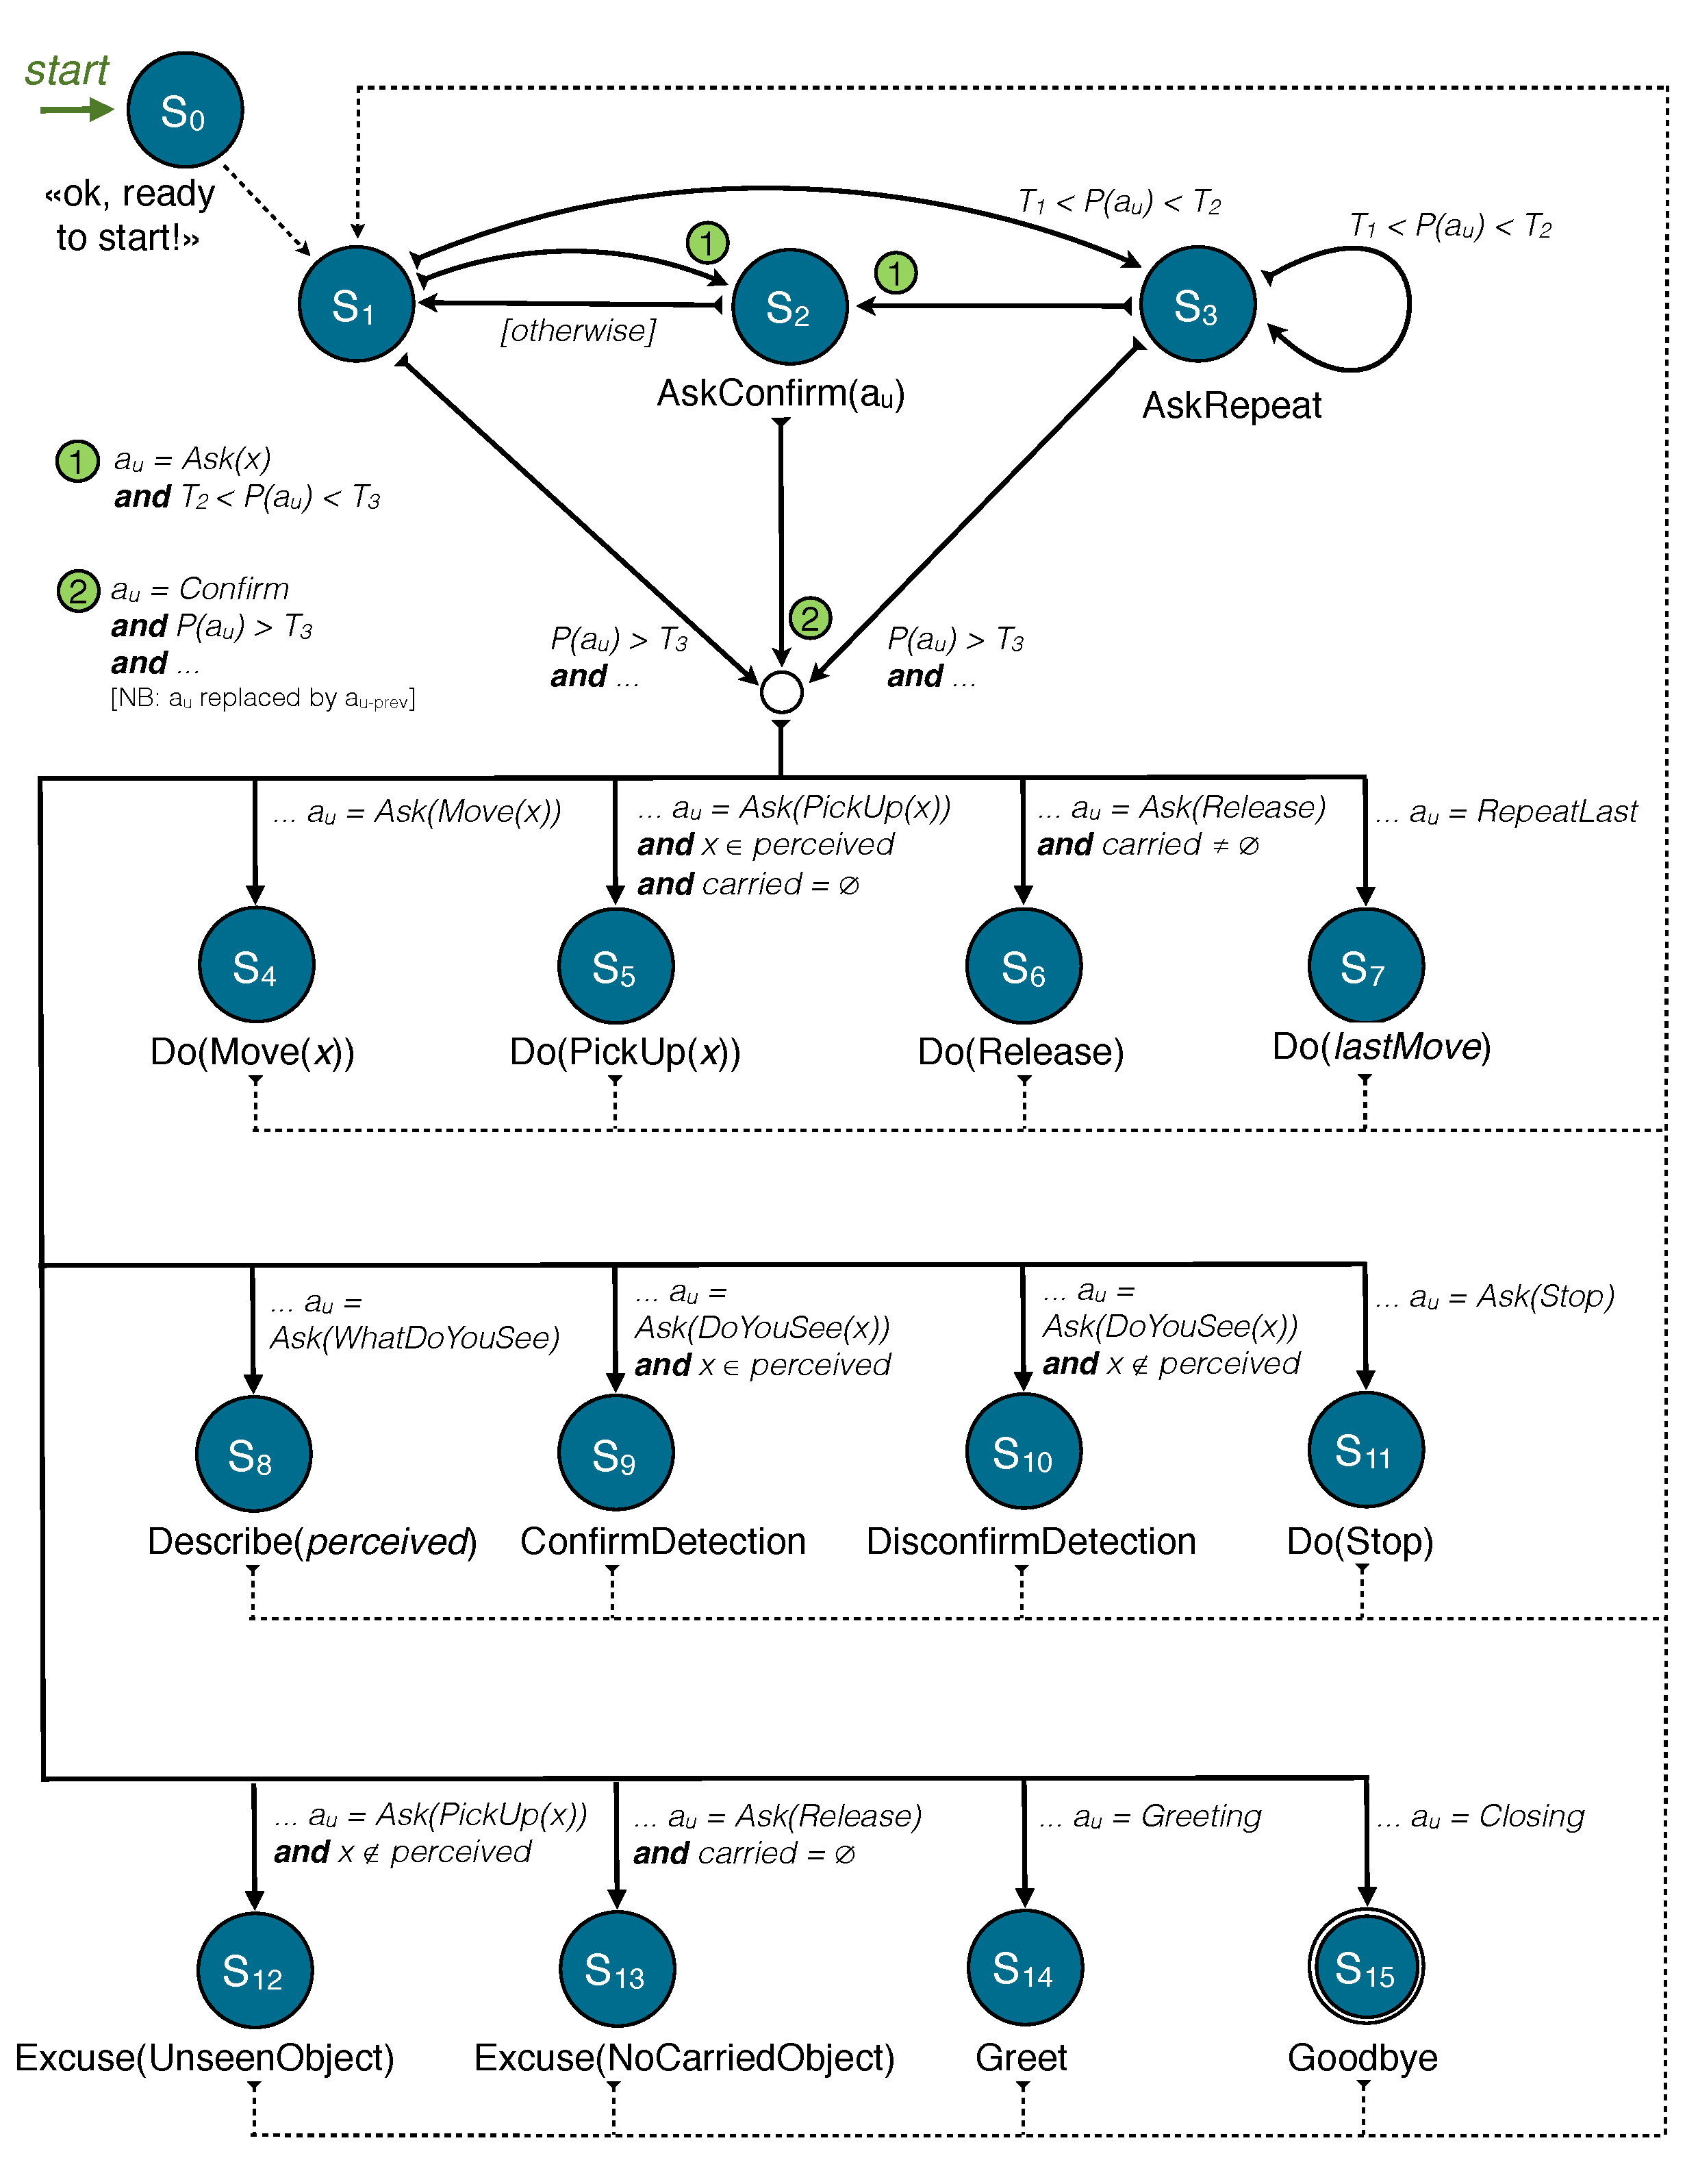
\includegraphics[scale=0.4]{imgs/fsa-exp3.pdf} 
\caption{Finite state automata designed for the domain (slightly simplified for clarity's sake). The dashed arrows denote empty transitions. For presentation purposes, the conditions applied to the edges going from $s_1,s_2,s_3$ to $s_4 \cdots s_{15}$ are decomposed in two parts: the first part from the incoming node to the small white circle, and the second part from the circle to the outgoing node. $T_1$, $T_2$ and $T_3$ are threshold values determined empirically.}
\label{fig:fsa-exp3}
\end{figure}


\subsubsection*{Probability thresholds}

The threshold values $T_1$, $T_2$ and $T_3$ are determined empirically on the basis of the actual probability values generated by the speech recogniser and NLU module during the Wizard-of-Oz study.  This estimation was achieved in two steps.  The first step consisted in  extracting all probability values associated with the most likely hypothesis of the user dialogue act $a_u$ in the recorded Wizard-of-Oz interactions and deriving a probability density from these values through kernel density estimation. The resulting density function is shown in Figure \ref{asrconfidence-exp3}. We then divided the distribution over probability values for the top user act hypothesis into four non-overlapping regions:
\begin{itemize}
\item The first region corresponds to user actions that most likely arise from spurious recognition and should hence be ignored. Based on a detailed inspection of the wizard actions in such cases, we mapped this region to the lowest quintile of the distribution (that is, all values with a cumulative density between $0$ and $0.2$). 
\item The second region corresponds to user actions that are more likely to reflect real user inputs, but do not have sufficient confidence to be directly executed.  This region was mapped to the second quintile of the distribution (values with a cumulative density between $0.2$ and $0.4$).
\item The third region corresponds to user actions that are relatively confident, but should nevertheless be confirmed once before execution.  This region was constrained to the third quintile of the distribution (values with a cumulative density between $0.4$ and $0.6$).
\item Finally, the fourth and final region corresponds to user actions that are sufficiently confident to be directly executed without user confirmation. This region defines the top 40 \% of the probability mass, with cumulative densities between $0.6$ and $1.0$.
\end{itemize}

The values that delineate these four regions can be calculated using linear interpolation. In practice, the estimated thresholds for the density function shown in Figure \ref{fig:asrconfidence-exp3} were derived to be $T_1 = 0.49$, $T_2 = 0.61$ and $T_3 = 0.73$. These values reflect the three thresholds employed in the finite state automaton. 


\begin{figure}[h!]
\centering
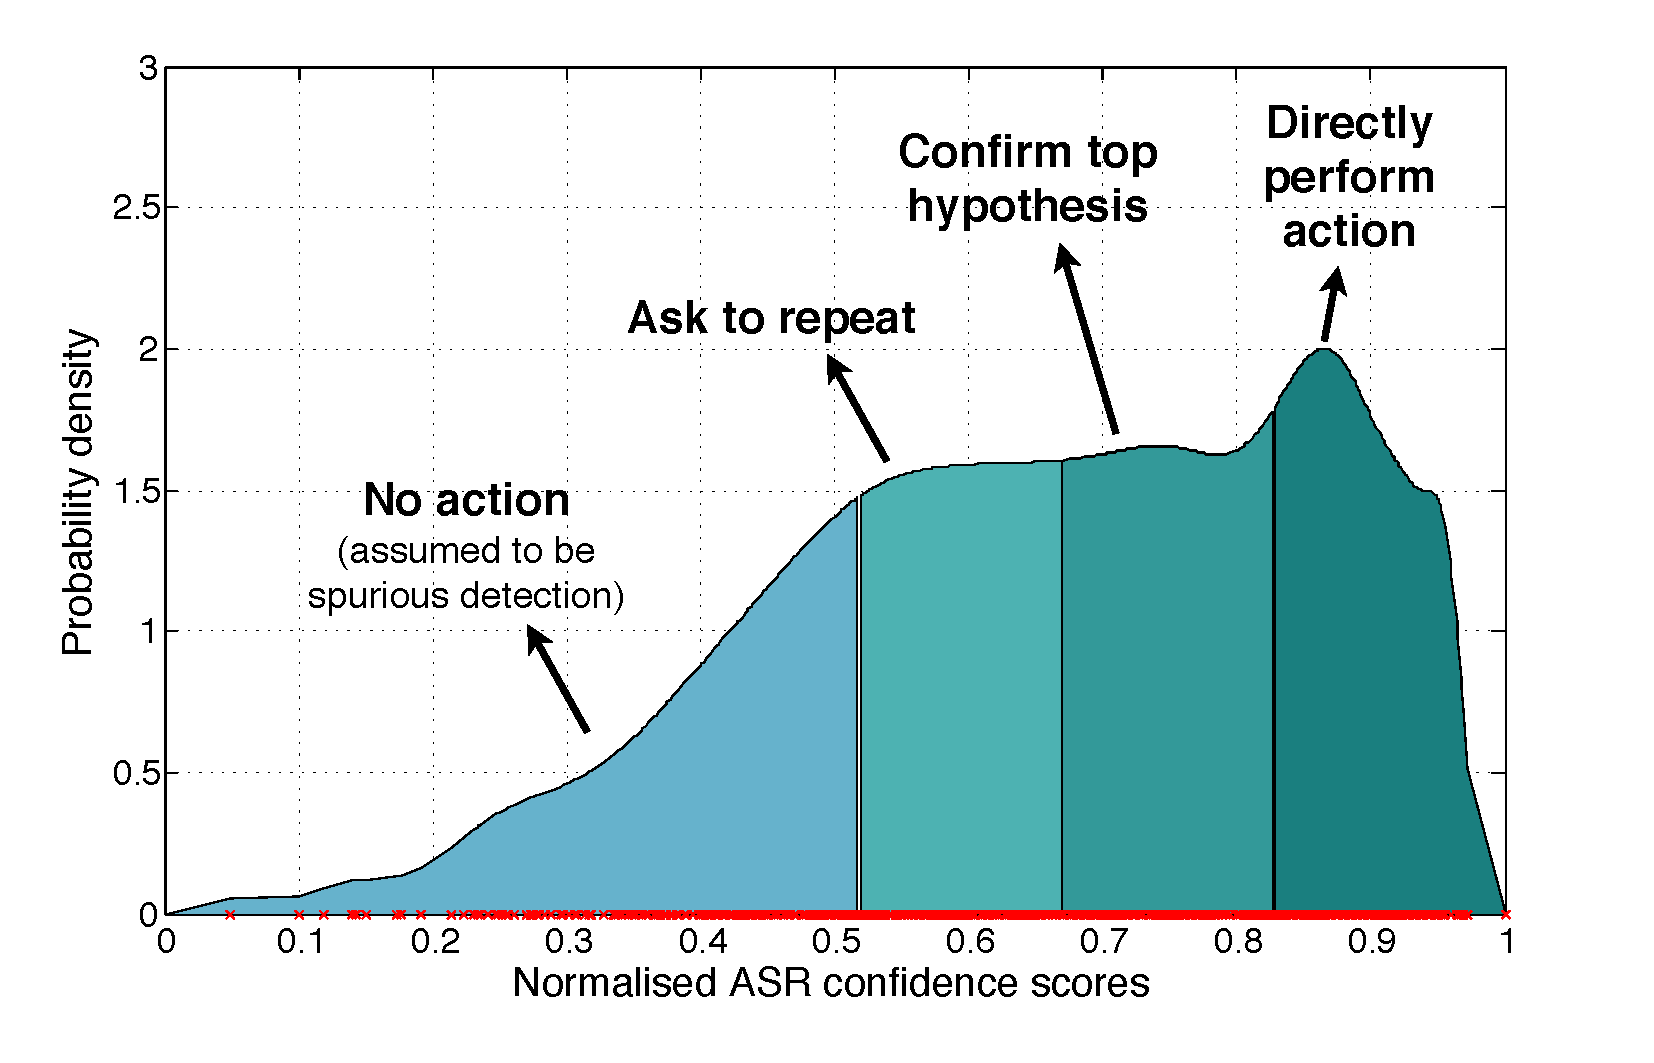
\includegraphics[scale=0.45]{imgs/asrconfidence.pdf} 
\caption{Probability density function for the probability values of the top hypothesis specified in the user dialogue act $a_u$, divided into four non-overlapping regions that respectively correspond to the first, second, third, and fourth+fifth quintiles of the distribution. The actual probability values are marked as red crosses on the X axis. }
\label{fig:asrconfidence-exp3}
\end{figure}


\subsection{Factored statistical model}

The second approach developed for this experiment consist of a traditional statistical model whose parameters are estimated from the Wizard-of-Oz data set collected for the experiment.  The parameter estimation is follows the Bayesian learning procedure presented in Chapter \ref{chap:wozlearning}. 

To reduce the problem of data sparsity, the model is factored in several smaller models. 

\subsection{Rule-structured model}

\subsection{Learning curves}

\section{User trials}

\subsection{Experimental setup}

\subsection{Metrics}


\note{various measures (number of turns, duration, number of disconfirm)}

\note{direct assessment of user satisfaction}

\subsection{Results}

\note{ANOVA, since we would have two baselines and our approach? (see e.g. Passonneau's article)}


\subsection{Analysis}

\section{Conclusion}




% note about our approach: generalisation enable a better account of the data sparsity problem.  plus, the state dynamics are not lost since we perform belief update.  Finally, the appraoch can be seen as an initial boostrapping that can then be further refined through online reinforcement learning (Bayesian prior), as in Williams etc. also, we learn utilities, not a direct classification. Also: a user simulator is difficult for situated and open-ended environments.  we learn a POMDP policy by simulation
